\chapter{FİZİBİLİTE}
Fizibilite araştırması; teknik, zaman, ekonomik ve yasal açıdan incelenmiştir.
Teknik fizibilite çalışmasında, uygulamanın yazılım, donanım ve iletişim ihtiyaçları
için; geliştirme, çalıştırma ve kullanma süreçlerindeki ihtiyaçlar belirlenmiş ve bu
ihtiyaçları karşılayacak en uygun çözümler bulunmuştur.
Zaman fizibilitesi çalışmasında, yapılacak iş listesi ve bunları gerçekleştirecek çalışanlar
belirlenmiş, zaman planlamasına yönelik gantt diyagramı oluşturulmuştur.
Ekonomik fizibilite çalışmasında, kullanılacak yazılım ve donanımların maliyetleri ile
çalışanlara ödenecek ücretler belirlenmiştir.
Yasal fizibilite çalışmasında, projenin gerçekleştirilmesinin önünde yasal bir engel olup
olmadığı araştırılmıştır.

\section{Teknik Fizibilite}
Teknik fizibilite çalışması Yazılım, Donanım ve İletişim fizibilitesi şeklinde 3 ana
başlık altında incelenecektir. Bunun yanı sıra her fizibilite çalışması kendi içinde
uygulamanın geliştirme süreci, çalıştırma süreci ve kullanıcının erişim süreci olarak 3
başlık altında incelenecektir.

\subsection{Yazılım Fizibilitesi}
Uygulama, sunucu-istemci mimarisine dayalı bir web uygulaması olacaktır. Genel
itibariyle Java teknolojileri kullanılacaktır.
 
Geliştirme Süreci \\
Uygulama Java EE kullanılarak MVC mimarisine uygun bir şekilde geliştirilmesi
planlanmıştır. MVC mimarisi yazılımda yeniden kullanılabilirliği artırır ve yazılımın
değişikliklere daha esnek hale gelmesini sağlar\cite{mvc}. Java EE’ ye en uygun alternatif
ASP.NET MVC' dir. ASP.NET platform bağımlı olması hem geliştirme hem de
uygulamayı çalıştırma sürecinde kısıtlayıcı rol oynayacaktır. Java teknolojilerinin tercih
edilmesinin temel sebebi ise, Java'nın açık kaynak kodlu, platform bağımsız, taşınabilir
ve (ilkel veri tipleri hariç) nesne yönelimli bir dil olmasıdır\cite{javaNesne}. Her ne kadar sahibi
Oracle olarak görülse de hem açık kaynak kodlu olması hem de gelişmelerin Oracle' ın6
tekelinde değil de JCP tarafından dünyanın her yerinden yazılımcıların katılımıyla
demokratik olarak sağlanması Java programlama dilini tercih edilir kılmıştır\cite{jcp}.
Java Servlet ve JSP birlikte MVC mimarisine uygun bir geliştirme imkanı
sağlamaktadır. Servlet ve JSP sunucu tarafında çalışır. Sevlet controller olarak, JSP ise
view olarak görev yapar. Her ikisi de sunum katmanındadır. Uygulama katmanında ise
model sınıfları olarak kullanılan EJB’ ler yer alır.
\\
Sunum katmanının kullanıcı arayüzü kısmında JSP ile beraber görsel öğeler ve bunların
düzenlenmesi için HTML ve CSS kullanılacaktır. Farklı web tarayıcıları HTML ve
CSS’
i
yorumlarken
farklı
varsayılan
değerler
kullandığından
görünümler
farklılaşabilmektedir. . Bu noktada, görsel tasarımın ortaklığını sağlamak amacıyla Eric
Meyer tarafından oluşturulan reset.css dosyası\cite{resetCSS} kullanılacaktır.
\\
IDE olarak Netbeans tercih edilmiştir. Netbeans' e alternatif olarak Eclipse ve IntelliJ
Idea gösterilebilir. Netbeans' in seçilme sebepleri ise şu şekilde sıralanabilir: Oracle gibi
güçlü bir geliştiricinin destek vermesi dolayısıyla Java SE ve EE yeni sürümlerinde
herhangi bir uyum sorununun yaşanmaması, arayüzünün swing ile geliştirilmesi
sebebiyle kaliteli bir kullanım sunması, web uygulamaları geliştirmede kullanılacak
diğer dillerle de ( JavaScript, HTML 5, CSS) uyumlu olması\cite{nedenNetbeans}. Netbeans 8.1
geliştirme amacıyla kullanılabilmesi için JRE 7 veya 8 ile, JDK 7 veya 8 üzerine ihtiyaç
duymaktadır\cite{netbeansJDKGereksinim}.
\\
Uygulama sunucusu olarak GlassFish seçilmiştir. Sunucu yazılımı tercih noktasında en
önemli alternatif Apache Tomcat olsa da, Tomcat sadece Servlet Container olarak görev
yapar, Java EE uygulama sunucusu olarak yetersizdir\cite{tomcat}.
\\
Veritabanı tercihi ilişkisel veritabanından yana kullanılmış ve PostgreSql seçilmiştir.
Veritabanı arayüzü için ise pgadmin III kullanılacaktır. PostgreSql 9.5 sürümü ile
birlikte çok daha kararlı, güvenli ve performanslı hale gelmiştir\cite{postgres}. Bu sürümün
getirdikleri PostgreSql'i diğer seçenekler arasından öne çıkarmıştır. PostgreSql arayüzü
için çok fazla seçenek bulunmaktadır\cite{postgresGUI}. Bunlar arasından pgadmin, karakter desteği,
yeterli dokümantasyona sahip olması ve sağladığı rutin bakımlar sebebiyle kullanılmak
üzere seçilmiştir\cite{pgAdmin}.
\\
Geliştirme sürecinde veritabanı işlemleri için Nesne-İlişkisel Eşlemeden (ORM)
faydalanılacaktır. Bununla veri tabanı işlemlerinin daha hızlı, performanslı ve düzenli
bir kod ile halledilmesi amaçlanmıştır\cite{ormNedir}. Aynı zamanda veri tipi uyumsuzluklarının7
da önüne geçilecektir. Java Community Process tarafından geliştirilen\cite{jpa} JPA(Java
Persistance API) arayüzü ve bunun Hibernate implementasyonu tercih edilecektir.
Native Hibernate, JPA arayüzünden önce geliştirilmiş, JPA arayüzü tanımlanınca onu
da destekler halde getirilmiştir. JPA' nın kalıtım desteği ve yeni sorgu metotlarını
destekler aynı zamanda yüksek performans, kararlılık ve ölçeklenebilirlik sergiler\cite{hibernateOrm}.
Geliştirme sürecinde ayrıca, Git sürüm kontrol sistemi ve Junit Java Test Çatısı'ndan
yararlanılacaktır. Sürüm kontrol sisteminin kullanılma amacı, yazılım sürecindeki
gelişmeleri takip edebilmek, gerekirse yapılan değişiklikleri geri alabilmek, yeni bir
özellik eklerken çalışmayı bozmayacak şekilde yan dallarla çalışma imkanı bulmaktır.
Merkezi sürüm kontrol sistemi yerine dağıtık bir sürüm kontrol sistemi olan Git' in
tercih edilme sebebi, hem yerel hem uzak depo avantajlarından faydalanmaktır\cite{git}.
Uygulamanın geliştirileceği işletim sistemi olarak Ubuntu seçilmiştir. Ubuntu geniş bir
topluluk tarafından desteklenen Linux çekirdeğini kullanmaktadır ve her 6 ayda bir yeni
sürüm çıkarma politikasına sahiptir. Ayrıca bu sürümlere 9 ay boyunca güvenlik ve hata
yamalarıyla beraber güncelleme desteği sunmaktadır\cite{ubuntuSurum}.
Geliştirme ve çalıştırma süreçlerinde farklı işletim sistemleri tercih edilecektir. Bunun
sebebi şöyle açıklanabilir. Ubuntu son kullanıcıya yönelik bir işletim sistemidir.
Yazılım geliştiricilerin bir yandan yazılımı geliştirirken diğer yandan mail
gönderme/okuma, internetten araştırma yapma, yazılımı test etme, telekonferanslara
katılma gibi günlük rutin işlerini devam etmelerine kolaylık sağlar. Sunucu işletim
sistemleri ise sunucular üzerindeki uygulamaların hizmet vermesine yönelik
tasarlanmıştır, son kullanıcı isteklerini yüksek performansta gerçekleştiremezler.


Çalıştırma Süreci\\
Çalıştırma sürecinde, geliştirme sürecinde olduğu gibi PostgreSQL ile ilişkisel
veritabanı yönetim sistemi ve Glassfish uygulama sunucusu kullanılacaktır. Güvenlik,
kararlılık, donanımı performanslı kullanma gibi sebeplerden dolayı\cite{serverKarsilastirma} Linux tabanlı
bir sunucu işletim sistemi kullanma kararı alınmıştır. Ayrıca açık kaynak kodlu olması
bir diğer avantajıdır. Paket yönetim kolaylığı, bakım periyodunun az olması ve Red Hat'
in geliştirme desteği gibi sebeplerle\cite{centos} Centos işletim sisteminde karar kılınmıştır.

Kullanma Süreci\\
Geliştirilen uygulama bir web uygulaması olduğundan dolayı, uygulamaya erişim için
herhangi bir web tarayıcı yeterli olacaktır.
Seçilen yazılımların, son kararlı sürümlerinin seçilmesine özen gösterilmiştir. Bu
açıdan, Netbeans EE 8.1, Java EE 7, GlassFish 4.1, PostgreSql 9.5, pgadmin 1.22,
Servlet 4.0, 2.3, Hiberbanate 5., CentOS 5, Ubuntu 15.04 kullanılacaktır.

\subsection{Donanım Fizibilitesi}
Uygun donanımın seçilebilmesi için önce donanım ihtiyaçları belirlenmelidir. Bu
amaçla yazılım fizibilitesinde belirlenen yazılımların en düşük sistem gereksinimleri,
geliştirme, çalıştırma ve kullanma süreçleri için ayrı ayrı belirlenmiştir.

Geliştirme Süreci\\

\begin{table}[]
\centering
\caption{Geliştirme Süreci İçin Yazılımların Minimum Sistem Gereksinimleri}
\label{my-label}
\begin{tabular}{|c|c|c|c|}
\hline
Yazılım Ürünü   & İşlemci                                                                                & Bellek  & Disk Alanı \\ \hline
Netbeans\cite{netbeansJDKGereksinim}        & \begin{tabular}[c]{@{}c@{}}800 MHz Intel \\ Pentium III ya da \\ eşdeğeri\end{tabular} & 512 MB  & 750 MB     \\ \hline
Java EE\cite{javaEEGereksinim}         & Özel bir şart yok                                                                      & 1024 MB & 250 MB     \\ \hline
Glassfish\cite{glassfishGereksinim}       & Özel bir şart yok                                                                      & 1024 MB & 250 MB     \\ \hline
Ubuntu\cite{ubuntuGereksinim}          & 1024 MHz                                                                               & 1536 MB & 7168 MB    \\ \hline
En düşük gereksinim & 1024 MHz                                                                               & 4 GB    & 8418 MB    \\ \hline
\end{tabular}
\end{table}

Tablo 3.2’de görüldüğü üzere geliştirme sürecinde kullanılacak yazılımların gerekli
donanım özellikleri piyasada bulunan standart değerlerin altındadır. Bu yüzden
tarafımca önerilen değerler Tablo 3.3’te belirtilmiştir.

\begin{table}[]
\centering
\caption{Geliştirme Süreci İçin Gerekli Yazılımların Önerilen Sistem Gereksinimleri}
\label{my-label}
\begin{tabular}{|c|c|c|}
\hline
İşlemci           & Bellek & Disk Alanı \\ \hline
1500 MHz Intel i5 & 4 GB   & 80 GB      \\ \hline
\end{tabular}
\end{table}

Çalıştırma Süreci \\
Çalıştırma sürecinde öncelikle sistemin kullanıcı sayısı tespit edilmeye çalışılmıştır. Ön
inceleme bölümünde 4 tip kullanıcı olduğu belirtilmişti. YTÜ Öğrenci İşleri Daire
Başkanlığı’nın internet sayfasındaki rapora göre \cite{ogrenciIstatistik} 2015-2016 Bahar Yarıyılı için YTÜ’
ne kayıtlı 35361 öğrenci vardır. YTÜ Teknopark’ a kayıtlı şirket sayısı ise 340’ tır\cite{teknoparkSirketler}.
Sistem yöneticisi ve BKB kullanıcıları bu rakamlar yanında ihmal edilebilir.

İhtiyaç duyulan disk kapasitesi kullanıcı profillerinin ve ilanların toplam boyutu düşünülerek 
hesaplanırsa; sks şirket kullanıcı sayısını, oks öğrenci kullanıcı sayısını, kbp kullanıcı profil büyüklüğünü (MB
cinsinden), ib ilan büyüklüğünü (MB cinsinden), ais ayda yayımlanan ilan sayısını göstermek üzere, 1 yıllık disk 
ihtiyacı:

(sks + oks) x kpb + ib x ais 

olarak hesaplanır. Bir yıldan sonraki süreçte, kullanıcı sayısı ilan sayısına oranla daha yavaş bir artış gösterecektir.

Öngörülen değerler ile ilk bir yılın tahmini disk ihtiyacı şöyle hesaplanmıştır:

sks = 340, oks = 17500 ( öğrencilerin yarısının sistemi kullanacağı düşünülmüştür), ib = 1(MB), kbp = 2(MB)  olmak üzere,

(340 + 17500) * 2 + 1 * 340 = 36020 (MB)

\begin{table}[]
\centering
\caption{Çalıştırma İçin Gerekli Yazılımların Minimum Sistem Gereksinimleri}
\label{my-label}
\begin{tabular}{|c|c|c|c|}
\hline
Yazılım Ürünü    & İşlemci             & Bellek            & Disk Alanı \\ \hline
Veritabanı       & Özel bir şart yok   & Özel bir şart yok & 36020 MB   \\ \hline
Glassfish        & Özel bir şart yok   & 1024 MB           & 250 MB     \\ \hline
CentOS           & Pentium III 450 MHz & 512 MB            & 5 GB       \\ \hline
En düşük ihtiyaç & Pentium III 450 MHz & 1.5 gb            & 40 GB      \\ \hline
\end{tabular}
\end{table}

Tablo 3.4’teki değerler göz önünde tutularak tarafımca önerilen değerler Tablo 3.5’te
verilmiştir.

\begin{table}[]
\centering
\caption{Çalıştırma Süresi İçin Gerekli Yazılımların Önerilen Sistem Gereksinimleri}
\label{my-label}
\begin{tabular}{|c|c|c|}
\hline
İşlemci                    & Bellek  & Disk Alanı \\ \hline
4 Çekirdek 1700 MHzişlemci & 8192 MB & 1 TB       \\ \hline
\end{tabular}
\end{table}

Kullanma Süreci\\
Uygulamanın iş yükü sunucu üzerinde olacağından (fat server-thin client) web tarayıcı
içeren ve internet bağlantısı sağlayabilen herhangi bir cihazla uygulamaya
erişilebileceğinden kullanım süreci için ayrıca bir donanım fizibilitesine gerek
duyulmamıştır.

\subsection{İletişim Fizibilitesi}
İletişim fizibilitesinde kullanıcıların sistem ile olan etkileşimleri ele alınmıştır.
Kullanıcıların uygulamayla etkileşimleri anlık bir süreklilik içerisinde değil, belirli
sayfaları görüntülemek sonrasında o sayfaları incelemek veya belirli formları
doldurduktan sonra bilgileri veritabanına göndermek ile sınırlı olacağından, sunucuya
bir anlık ağ görüntüsünde gelen istek ve dönen cevapların çok fazla olmayacağı
düşünülmüştür.\\

Sistemde anlık 10000 kullanıcı olacağı ve bu kullanıcılardan \%5’ inin bir anda istek
göndereceği düşünülmüştür. Gelen istekler daha çok ilan görüntüleme üzerine olacaktır.
Bu yüzden gelen isteklerin boyutu az fakat sunucudan dönen cevap boyutu büyük
olacaktır.
Gelen istekler bir ilanın görüntülenmesi, ilan yüklenmesi veya profil bilgilerinin
değiştirilmesi olabilir. Ortalama bir isteğin boyutu 10 KB alınmıştır.
Anlık kullanıcı sayısı aks, anlık aktif kullanıcı oranı aaks, bir kullanıcıdan gelen ortalama istek boyutu D olmak üzere:

İndirme hızı = aks * aaks * D

İndirme hızı = 10000 * 0,05 * 10 KB

Yaklaşık 5 MB anlık istek boyutu bulunur. Sunucumuzun bu en kötü senaryoda 2 saniyelik bir gecikme ile istekleri karşılayacağını düşünürsek 2,5 Mbps indirme hızını karşılayabilmesi gerektiğini söyleyebiliriz.

Yükleme miktarı da aynı formülle hesaplanır. Fakat cevap boyutu daha fazla, anlık
kullanıcı sayısı ise daha az olacaktır. Çünkü ilanların incelenmesi, sık istek gönderilen
bir durum değildir. Kullanıcıların \%0,5’ inin aynı anda bir ilanı görüntülemek için istek
gönderdiği, 1 isteğin de 1MB olacağı düşünülürse:

Yükleme hızı = 10000 * 0,005 * 1 MB

Yaklaşık 50 MB anlık istek boyutu olarak hesaplanır. En kötü senaryomuzun yine 2 saniye sürede işlenebilmesi için,
sunucumuzun bant genişliğinin saniyede ortalama 25 MB' lık veri gönderimini karşılayabilecek seviyede olması gerekir.

Sunucu, kullanıcılardan sorunsuzca istek alabilmek için 2.5Mbps indirme hızını,
isteklere cevap verebilmek için 25 Mbps yükleme hızına sahip olmalıdır.
Son kullanıcıların sunuyla haberleşebilmeleri için internet bağlantısı sağlayabilen bir
cihaza sahip olmaları gerekmektedir. Ortalama istek boyutunu 10 KB, cevap boyutunu 1MB varsaymıştık, Günümüz 
İnternet hızlarını düşündüğümüzde bu boyutlar hızlıca yüklenebilecek değerdedir. En kötü senaryonun yaşanmadığı bir zaman için
1Mbps hızına sahip kullanıcıların iyi bir kullanıcı deneyimine sahip olacaklarını söyleyebiliriz.

\section{Zaman Fizibilitesi}
Proje geliştirme sürecinde görev alacak çalışan rolleri, çalışan sayıları ve görev
kapsamları Tablo 3.6’ da verilmiştir. Zaman planlamasına ilişkin Gantt diyagramı Şekil
3.1’ de, Gantt diyagramına ait zaman-çalışan tablosu ise Tablo 3.7’de verilmiştir.

\begin{table}[]
\centering
\caption{Projede yer alan çalışan rolleri, sayıları ve görev tanımları}
\label{my-label}
\begin{tabular}{|c|c|c|}
\hline
Rol                                                                  & Çalışan Sayısı & Görev                                                                                                                                                          \\ \hline
Proje Yöneticisi                                                     & 1              & \begin{tabular}[c]{@{}c@{}}Projenin her aşamasından sorumludur.\\ Aynı zamanda ön inceleme, fizibilite ve\\ sistem analizi aşamalarını gerçekler.\end{tabular} \\ \hline
Yazılım Mimarı                                                       & 1              & \begin{tabular}[c]{@{}c@{}}Ön incelemeye bağlı olarak sistem tasarımını\\ (veritabanı ve nesneye yönelik tasarım) yapar.\end{tabular}                          \\ \hline
\begin{tabular}[c]{@{}c@{}}Uygulama\\ Geliştirme Uzmanı\end{tabular} & 2              & \begin{tabular}[c]{@{}c@{}}Yazılım Mimarı' nın ortaya koyduğu \\ tasarıma bağlı olarak \\ kodun yazılmasından sorumludur.\end{tabular}                         \\ \hline
Test Sorumlusu                                                       & 2              & \begin{tabular}[c]{@{}c@{}}Uygulama Geliştirme Uzmanı’ nın \\ yazdığı kodun birim ve entegrasyon \\ testlerini yapar.\end{tabular}                             \\ \hline
\begin{tabular}[c]{@{}c@{}}Ön yüz Geliştirme\\ Uzmanı\end{tabular}   & 1              & \begin{tabular}[c]{@{}c@{}}Gerçeklenen işlevlerin kullanımı için,\\ kullanıcı dostu bir arayüz geliştirir.\end{tabular}                                        \\ \hline
\end{tabular}
\end{table}

% Please add the following required packages to your document preamble:
% \usepackage[normalem]{ulem}
% \useunder{\uline}{\ul}{}
\begin{table}[]
\centering
\caption{Görev-Rol-Zaman}
\label{my-label}
\begin{tabular}{|c|c|c|}
\hline
Görev Adı             & Ana Sorumlu                                                          & Süresi (gün) \\ \hline
Ön İnceleme           & Proje Yöneticisi                                                     & 3            \\ \hline
Fizibilite            & Proje Yöneticisi                                                     & 5            \\ \hline
Sistem Analizi        & Proje Yöneticisi                                                     & 1            \\ \hline
Sistem Tasarımı       & Yazılım Mimarı                                                       & 6            \\ \hline
İşlevlerin Kodlanması & \begin{tabular}[c]{@{}c@{}}Uygulama Geliştirme\\ Uzmanı\end{tabular} & 12           \\ \hline
Testlerin Yapılması   & Test Sorumlusu                                                       & 12           \\ \hline
GUI Geliştirme        & \begin{tabular}[c]{@{}c@{}}Ön-yüz geliştirme\\ uzmanı\end{tabular}   & 8            \\ \hline
Kullanıcı Kabul Testi & Proje Yöneticisi                                                     & 1            \\ \hline
\end{tabular}
\end{table}

\begin{figure}[]
    \centering
        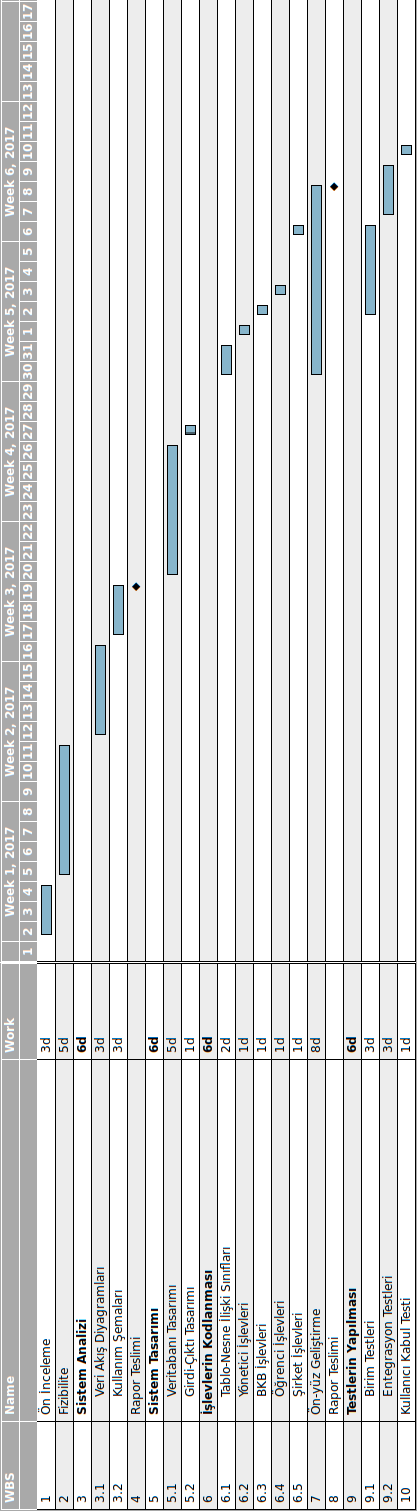
\includegraphics[width=.90\textwidth]{projectChapters/images/gantt.png}
    \caption{Gantt Çizelgesi}
    \label{ganttLabel}
\end{figure}

\section{Yasal Fizibilite}

Kullanılan yazılım ürünlerinin lisansları Tablo 3.8’ de verilmiştir. Lisanların
incelenmeleri sonucunda kullanım için bir engele rastlanmadığı görülmüştür. Lisans bedeli ücretli olan MS Visio
Ekonomik Fizibilite bölümünde ele alınmıştır.

\begin{table}[]
\centering
\caption{Kullanılan Yazılım Ürünlerinin Lisansı}
\label{my-label}
\begin{tabular}{|c|c|}
\hline
Yazılım Ürünü & Lisansı                                     \\ \hline
Netbeans\cite{netbeansLisans} & Common Development And Distribution License\cite{cddl} \\ \hline
Glassfish\cite{glassfishLisans}     & Common Development And Distribution License\cite{cddl} \\ \hline
Ubuntu\cite{ubuntuLisans}        & General Public License{gpl}                      \\ \hline
Centos        & General Public License\cite{gpl}                      \\ \hline
Java EE       & Java Development License\cite{jdl}                    \\ \hline
\end{tabular}
\end{table}


Gelir Vergisi Kanunu’ nun 89/2 maddesine göre\cite{vergi}, şirket kazancının \%5’ ini
geçmemek kaydıyla ve makbuz karşılığı yapılan bağışlar vergiden düşülür. Bu
bağışların yapılabileceği kurumlar arasında üniversitemiz bilimsel araştırma yapılan
kurumlar dahilinde olup, söz konusu olan makbuz şartını, bağış kabul eden birimlerince
verebilmektedir. \\
Şirketlere sunulacak hizmet, yapılacak bağış karşılığında, belirlenen süre ve adete bağlı
olarak sistem üzerinden ilan yayınlama hakkı verir. Eğer ilanlar, kişi ve kurumların
itibarını zedeleyici unsurlar içeriyorsa yayından kaldırılır ve şirkete yeni bir ilan
yayınlama hakkı verilmez. Sistem ayrıca erişilebilirlik için mümkün olan en yüksek
performansla çalışır fakat, sunucu veya ağ hizmetlerinden doğabilecek sorunlar
karşılığında sorumluluk kabul edilmez.

\section{Ekonomik Fizibilite}
Öncelikle teknik, yasal ve ekonomik fizibilitelerin kendi içerisinde maliyet hesaplamaları yapılmış, sonrasında ise
toplam maliyet çıkarılmıştır.

\subsection{Teknik Fizibiliteden Doğacak Giderler}
Yazılım fizibilitesi kapsamında kullanılması belirlenen yazılımlardan sadece MS Visio
2016 ücretli olup, bu ücret 999 TL’dir\cite{visio}.
Donanım fizibilitesi kapsamında ise bir sunucu ihtiyacı tespit edilmiş olup, bu sunucu
satın alınabilir ya da bir hosting firması üzerinden kiralanabilir.
Sunucu satın alma seçeneği için yapılan araştırmalar sonucu IBM ' ait bir sunucu
kullanılmasına karar verilmiştir. Bunun temel sebebi aynı özellikteki çeşitli sunucuların
karşılaştırılması sonucunda fiyat/performans olarak IBM sunucuların daha iyi olmasıdır.
\cite{ibmKarsilastirma} Buradan görüleceği gibi HP, Intel, Power 8 ve IBM'in yer aldığı karşılaştırmada
IBM \$21.88 ile en iyisidir. Bir diğer karşılaştırma IBM ve Oracle arasında yapılmıştır.
Bu karşılaştırma sonucunda Oracle çeşitli zayıflıkları \cite{ibmvsOracle}(Dosya yönetimi, bulut
entegrasyonu, B2B bütünlüğü vs) sebebiyle seçenekler arasından elenmiştir. IBM
sunucuları arasından ihtiyaçlarımız doğrultusunda seçenekler taranmış, sistemin
genişleyebileceği düşünülerek karar verilmiştir. Bu karar IBM SRV 7383K7G ürünü
lehindedir. Bu ürün genel olarak şu özelliklere sahiptir: İşlemci: Intel Xeon E5 2.1 GHz,
Bellek 8GB( artırılabilir), Disk 3*300 GB(artırılabilir)\cite{ibmFiyat}. Seçilen IBM sunucu için
ödenecek ücret ise 7.663,17 TL'dir\cite{ibmFiyat}.
Hosting kiralama seçeneği için farklı firmaların sunduğu hizmetler incelenmiş ve Tablo
3.9’ da karşılaştırılmıştır. Buna göre İsim Tescil firmasından alanı adı, Reseller Hosting
firmasından ise hosting temini en uygun seçimdir.

% Please add the following required packages to your document preamble:
% \usepackage{graphicx}
\begin{table}[]
\centering
\caption{Hosting firmalarının sunduğu hizmetler ve fiyatları}
\label{my-label}
\resizebox{\textwidth}{!}{%
\begin{tabular}{|c|r|c|c|c|c|}
\hline
Firma Adı        & \multicolumn{1}{c|}{\begin{tabular}[c]{@{}c@{}}Fiyat (TL)\\ (Yıllık)\end{tabular}} & \begin{tabular}[c]{@{}c@{}}Web Alanı\\ (GB)\end{tabular} & \begin{tabular}[c]{@{}c@{}}Trafik(Aylık)\\ (GB)\end{tabular} & \begin{tabular}[c]{@{}c@{}}E Posta\\ Depolama Miktarı\\ (GB)\end{tabular} & \begin{tabular}[c]{@{}c@{}}Alan Adı\\ Kullanabilme Adedi\end{tabular} \\ \hline
Reseller Hosting\cite{reseller} & 99.99                                                                              & 60                                                       & 60                                                           & Sınırsız                                                                  & Sınırsız                                                              \\ \hline
Natro\cite{natro}            & 278,35                                                                             & Sınırsız                                                 & Sınırsız                                                     & Sınırsız                                                                  & 10                                                                    \\ \hline
Strato\cite{strato}           & 111,35                                                                             & 250                                                      & Sınırsız                                                     & 40                                                                        & 1                                                                     \\ \hline
İsim Tescil\cite{isimtescil}      & 695,96                                                                             & 100                                                      & Trafik                                                       & 6 (Alan Adı Başına)                                                       & 100                                                                   \\ \hline
\end{tabular}%
}
\end{table}

\subsection{Yasal Fizibiliteden Doğabilecek Giderler}
Yasal fizibiliteden doğacak herhangi bir gider bulunmamıştır.

\subsection{Ekonomik Fizibiliteden Doğacak Giderler}
Projede görev alacak çalışanlar, sayıları, günlük ve toplam ücretleri Tablo 3.10’ da
verilmiştir.

Projenin toplam maliyeti Tablo 3.11' de görüleceği üzere 10.257,35 TL olarak hesaplanmıştır.
\begin{table}[]
\centering
\caption{Görev-zaman-ücret-hesabı}
\label{my-label}
\begin{tabular}{|c|r|r|r|r|}
\hline
Çalışan Rolü                                                         & \multicolumn{1}{l|}{\begin{tabular}[c]{@{}l@{}}Çalışan \\ Sayısı\end{tabular}} & \multicolumn{1}{c|}{\begin{tabular}[c]{@{}c@{}}Çalışma Süresi\\ (Gün)\end{tabular}} & \multicolumn{1}{c|}{\begin{tabular}[c]{@{}c@{}}Günlük Ücret\\ (TL)\end{tabular}} & \multicolumn{1}{c|}{\begin{tabular}[c]{@{}c@{}}Toplam Ücret\\ (TL)\end{tabular}} \\ \hline
Proje Yöneticisi                                                     & 1                                                                              & 22                                                                                  & 150                                                                              & 3.300                                                                            \\ \hline
Yazılım Mimarı                                                       & 1                                                                              & 6                                                                                   & 120                                                                              & 720                                                                              \\ \hline
\begin{tabular}[c]{@{}c@{}}Uygulama Geliştirme\\ Uzmanı\end{tabular} & 2                                                                              & 12                                                                                  & 100                                                                              & 2.400                                                                            \\ \hline
Test Sorumlusu                                                       & 2                                                                              & 12                                                                                  & 80                                                                               & 1.920                                                                            \\ \hline
\begin{tabular}[c]{@{}c@{}}Ön-yüz Geliştirme\\ Uzmanı\end{tabular}   & 1                                                                              & 8                                                                                   & 80                                                                               & 640                                                                              \\ \hline
Toplam                                                               & \multicolumn{4}{r|}{8.980}                                                                                                                                                                                                                                                                                                                 \\ \hline
\end{tabular}
\end{table}

\begin{table}[]
\centering
\caption{Toplam Maliyet}
\label{my-label}
\begin{tabular}{|c|r|}
\hline
Gider Adı        & \multicolumn{1}{c|}{Maliyet (TL)} \\ \hline
Hosting          & 278,35                            \\ \hline
MS Visio         & 999                               \\ \hline
Çalışan Maliyeti & 8.980                             \\ \hline
Toplam           & 10.257,35                         \\ \hline
\end{tabular}
\end{table}
